% Created 2021-08-16 Mon 17:10
% Intended LaTeX compiler: pdflatex
\documentclass[bigger]{beamer}
\usepackage[utf8]{inputenc}
\usepackage[T1]{fontenc}
\usepackage{graphicx}
\usepackage{grffile}
\usepackage{longtable}
\usepackage{wrapfig}
\usepackage{rotating}
\usepackage[normalem]{ulem}
\usepackage{amsmath}
\usepackage{textcomp}
\usepackage{amssymb}
\usepackage{capt-of}
\usepackage{hyperref}
\mode<beamer>{\useinnertheme{rounded}\usecolortheme{rose}\usecolortheme{dolphin}\setbeamertemplate{navigation symbols}{}\setbeamertemplate{footline}[frame number]{}}
\mode<beamer>{\usepackage{amsmath}\usepackage{ae,aecompl,sgamevar,tikz}}
\let\oldframe\frame\renewcommand\frame[1][allowframebreaks]{\oldframe[#1]}
\setbeamertemplate{frametitle continuation}[from second]
\newcommand{\Ra}{\Rightarrow} \newcommand{\ra}{\rightarrow} \newcommand{\Lra}{\Leftrightarrow}
\usetheme{default}
\author{Christoph Schottmüller}
\date{}
\title{Adverse selection}
\hypersetup{
 pdfauthor={Christoph Schottmüller},
 pdftitle={Adverse selection},
 pdfkeywords={},
 pdfsubject={},
 pdfcreator={Emacs 27.2 (Org mode 9.4.4)}, 
 pdflang={English}}
\begin{document}

\maketitle
\begin{frame}{Outline}
\tableofcontents
\end{frame}



\section{Introduction}
\label{sec:org18d3d17}
\begin{frame}[label={sec:orge1d6970}]{Introduction}
\begin{itemize}
\item markets can efficiently aggregate (private) information on willingness to pay and costs
\item today:
\begin{itemize}
\item private information on product feature
\item buyers cannot distinguish products with different features at the time of purchase
\item market incompleteness: goods with distinct features are traded on same market
\item first fundamental theorem of welfare economics does not apply
\end{itemize}
\end{itemize}
\end{frame}
\begin{frame}[label={sec:org17736a7}]{Adverse selection: basic idea I}
\begin{itemize}
\item sellers of used cars know something about the quality of their car that buyers do not know
\item sellers' reservation price for a high quality car is higher than for a low quality car
\item at every market price \(p\) only \(S(p)\) \emph{worst} cars will be offered ("adverse selection")
\item buyers' anticipate adverse selection
\begin{itemize}
\item willing to pay is low as anticipated quality is low
\item market breakdown as sellers are not willing to sell at these low prices
\end{itemize}
\end{itemize}
\end{frame}

\begin{frame}[label={sec:org1dd473d}]{Adverse selection: basic idea II}
\begin{itemize}
\item details of market breakdown logic:
\begin{itemize}
\item say \(S\) worst cars are offered
\item expected quality is average quality of offered cars
\item willingness to pay is average willingness to pay for cars of offered qualities
\item marginal seller (i.e. highest offered quality) may rather keep his car at such low price
\begin{itemize}
\item \(\Ra\) \(S-1\) cars offered
\item \(\Ra\) average quality even lower
\item \(\Ra\) willingness to pay even lower
\item \(\Ra\) another seller may decide not to sell
\item \dots{}
\end{itemize}
\end{itemize}
\end{itemize}
\end{frame}
\section{Simple model}
\label{sec:orgc3ccec1}
\begin{frame}[label={sec:orgb094999}]{Simple model}
\begin{itemize}
\item continuum of sellers 
\begin{itemize}
\item uniform distribution on \([0,1]\)
\item each seller \(i\in[0,1]\) owns 1 car of quality \(i\)
\item reservation utility of seller \(i\) equals \(i\)
\end{itemize}
\item continuum of buyers
\begin{itemize}
\item mass 1 of risk neutral buyers
\item each buyer \(j\) wants to buy 1 car
\item willingness to pay for a car of quality \(i\) equals \(\alpha i\) with \(\alpha>1\)
\end{itemize}
\item seller \(i\) knows the quality of his car
\item buyers cannot distinguish qualities at the time of purchase
\item equilibrium: a price \(p\) such that supply equals demand at this price
\end{itemize}
\end{frame}

\begin{frame}[label={sec:orgf1e9dec}]{Analysis: supply and demand}
\alert{Supply:}
\begin{itemize}
\item at price \(p\), all sellers \(i\leq p\) offer their car
\end{itemize}
$$S(p)=\begin{cases}p&\text{ if }p\in[0,1]\\1&\text{ if }p>1\end{cases}$$ 
\begin{itemize}
\item average offered quality at price \(p\) equals \(Q(p)=p/2\)
\end{itemize}


\alert{Demand:}
\begin{itemize}
\item at price \(p\in[0,1]\) quality offered equals \(Q(p)=p/2\)
\begin{itemize}
\item willingness to pay is above price if \(\alpha p/2\geq p\)
\item at price \(p>1\) average quality equals \(Q(p)=1/2\)
\end{itemize}
\end{itemize}
\begin{equation*}
D(p) = \begin{cases}1 & \text{ if }\alpha \geq 2 \text{ and }p\leq \alpha/2\\ 0 & \text{ else. } \end{cases}
\end{equation*}
\end{frame}

\begin{frame}[label={sec:orgf364451}]{Analysis: equilibrium}
\begin{itemize}
\item If \(\alpha\geq 2\), any \(p\in[1,\alpha/2]\) is an equilibrium price at which all cars are sold.
\item If \(\alpha<2\), no car is sold in equilibrium as demand is zero at any price. \linebreak
\(\Ra\) \(p=0\) is the equilibrium price at which demand and supply equal 0
\end{itemize}
\end{frame}


\begin{frame}[label={sec:orgbfa4a49}]{Results and discussion}
\begin{itemize}
\item asymmetric information on product features can lead to market failure (if gains from trade are not too large)
\item it is not clear how a government could beneficially intervene in such a failed market unless the government knows the qualities of the cars
\item key assumption: sellers are most reluctant to sell those cars that buyers value most
\item what practical measures are or could be taken in used car/goods markets to avoid market failure due to asymmetric information?
\end{itemize}
\end{frame}

\section{Insurance market model}
\label{sec:orgdf91013}
\begin{frame}[label={sec:org15011c1}]{Insurance market: basic idea}
\begin{itemize}
\item who has the higher willingness to pay for comprehensive health insurance: a chronically ill person (diabetes, HIV\dots{}) or a healthy person?
\pause
\item at any premium \(p\), the \(D(p)\) least healthy people will buy insurance
\item the least healthy cause the highest costs to insurance companies
\item "death spiral of health insurance":
\begin{itemize}
\item healthiest do not buy insurance
\item average cost for insurance go up
\item premium increase
\item healthiest of the still insured cancel their insurance
\item repeat
\end{itemize}
\end{itemize}
\end{frame}

\begin{frame}[label={sec:org1492799}]{Insurance market: model I}
\begin{itemize}
\item market for full insurance (all health care expenditures are covered 100\%)
\item continuum of consumers
\begin{itemize}
\item mass 1
\item consumer \(i\) has expected health care expenditures (when insured) of \(i\)
\item consumer values insurance \(\alpha i\) with \(\alpha>1\) (due to risk aversion)
\item consumers are distributed on \([i_l,i_h]\) with distribution \(F\) (and density \(f\))
\end{itemize}
\item perfectly competitive insurance market
\begin{itemize}
\item insurances have no administrative or other fixed costs
\item insurances maximize profit
\item \(\Ra\) an insurance's profit from insuring consumer \(i\) at premium \(p\) equals \(p-i\)
\end{itemize}
\end{itemize}
\end{frame}
\begin{frame}[label={sec:orgd395a66}]{Insurance market: model II}
\begin{itemize}
\item \emph{information:}
\begin{itemize}
\item consumers observe their risk \(i\)
\item insurances do not observe \(i\)
\end{itemize}
\item \emph{equilibrium:}
\begin{itemize}
\item premium \(p\) equals average cost of insured (due to perfect competition among insurance companies)
\item insured are those consumers whose value is above premium
\end{itemize}
\end{itemize}
\end{frame}

\begin{frame}[label={sec:org0eb87dc}]{Insurance market: analysis}
\emph{Demand:}
\begin{itemize}
\item at premium \(p\) all consumers \(i\) for which \(\alpha i\geq p\) buy insurance
$$D(p)=1-F(p/\alpha)$$
\item expected costs of insured are \(\mathbb{E}[i|i\geq p/\alpha]\)
\begin{itemize}
\item note: \(\mathbb{E}[i|i\geq p/\alpha]\) is increasing in \(p\) ("adverse selection")
\end{itemize}
\end{itemize}

\emph{Equilibrium:}
\begin{itemize}
\item in equilibrium
$$p=\mathbb{E}[i|i\geq p/\alpha]$$
solving this equation for \(p\) yields the equilibrium price \(p^*\)

\item let \(\hat i=p^*/\alpha\) be the marginal consumer
\begin{itemize}
\item if \(\alpha i_l<\mathbb{E}[i]\), then some consumers will not buy insurance
\end{itemize}
\end{itemize}


\emph{Welfare:}
\begin{itemize}
\item welfare maximizing to have everyone insured
\item adverse selection leads to underinsurance if \(\alpha i_l<\mathbb{E}[i]\)
\end{itemize}
\end{frame}
\begin{frame}[label={sec:org3aaa6e5}]{Insurance market: graph I}
\begin{figure}[h]
\centering
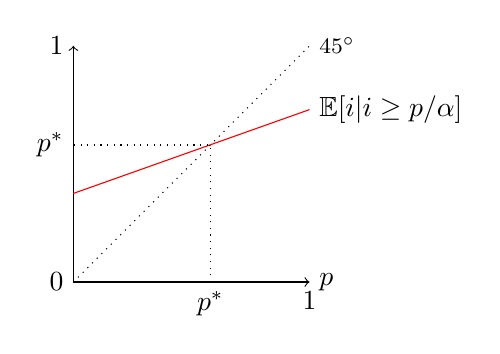
\begin{tikzpicture}[scale=3]
\draw[<->] (1,0)--(0,0)--(0,1);
\node[right] at (1,0) {$p$};
\draw[red] (0,.375)--(1,0.73);
\node[right] at (1,0.73) {$\mathbb{E}[i|i\geq p/\alpha]$};
\node[left] at (0,1) {$1$}; 
\node[left] at (0,0) {$0$};
\node[left] at (0,0.58) {$p^*$};
\node[below] at (1,0) {$1$};
\node[below] at (0.58,0) {$p^*$};
\draw[dotted] (0.58,0)--(0.58,0.58)--(0,0.58);
\draw[dotted] (0,0)--(1,1);
\node[right] at (1,1) {\footnotesize$45^\circ$};
\end{tikzpicture}
%
% \caption{Figure for $i$ uniformly distributed on $[1/4,3/4]$ and $\alpha=3/2$ implying $\mathbb{E}[i|i\geq\alpha p]=3/8+p/3$, $MC(q)=3/4-q/2$, $P(q)=1.125-3q/4$, $AC(q)=3/4-q/4$. Equilibrium: $p=9/16$, $\hat i=3/8$, $q=3/4$.}
\end{figure}
\end{frame}

\begin{frame}[label={sec:orgf1b2dd0}]{Insurance market: graph II}
similar to regular supply and demand diagram:
\begin{itemize}
\item marginal cost when quantity \(q\) is traded: \(MC(q)=F^{-1}(1-q)\)
\item average cost: \(AC(q)=\mathbb{E}[i|i\geq F^{-1}(1-q)]\)
\item inverse demand (i.e willingness to pay of marginal consumer): \(P(q)=\alpha F^{-1}(1-q)\)
\item equilibrium is intersection of \(P\) and \(AC\)
\item where is the welfare loss due to underinsurance depicted?
\end{itemize}

\begin{figure}
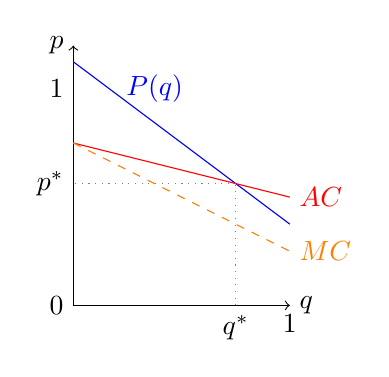
\begin{tikzpicture}[scale=2.75]
\draw[<->] (1,0)--(0,0)--(0,1.2);
\node[left] at (0,1.2) {$p$};
\node[right] at (1,0) {$q$};
\draw[blue] (0,1.125)--(1,0.375);
\node[right,blue] at (0.2,1) {$P(q)$};
\draw[red] (0,0.75)--(1,0.5);
\node[right,red] at (1,0.5) {$AC$};
\draw[orange,dashed] (0,0.75)--(1,0.25);
\node[right,orange] at (1,0.25) {$MC$};
\node[left] at (0,1) {$1$}; 
\node[left] at (0,0) {$0$};
\node[left] at (0,0.5625) {$p^*$}; %{$9/16$};
\node[below] at (1,0) {$1$};
\node[below] at (0.75,0) {$q^*$}; %{$3/4$};
\draw[dotted,gray] (0.75,0)--(0.75,0.5625);
\draw[dotted,gray] (0.75,0.5625)--(0,0.5625);
\end{tikzpicture}
% \caption{Figure for $i$ uniformly distributed on $[1/4,3/4]$ and $\alpha=3/2$ implying $\mathbb{E}[i|i\geq\alpha p]=3/8+p/3$, $MC(q)=3/4-q/2$, $P(q)=1.125-3q/4$, $AC(q)=3/4-q/4$. Equilibrium: $p=9/16$, $\hat i=3/8$, $q=3/4$.}
\end{figure}
\end{frame}

\begin{frame}[label={sec:orgf229cb3}]{Insurance market: policy}
\begin{itemize}
\item Who will benefit/lose from \emph{mandatory insurance} at premium \(\mathbb{E}[i]\)?

\begin{itemize}
\item Does this fit the lines of support for mandatory health insurance in the US?
\end{itemize}
\item Governments often \emph{subsidize} health insurance (using tax revenue).
\begin{itemize}
\item How does a subsidy affect welfare?
\item Does this per se justify such subsidies?
\end{itemize}
\end{itemize}

\begin{itemize}
\item The Affordable Care Act in the US originally included \emph{financial penalties} for those not buying health insurance.
\begin{itemize}
\item What are the effects of this policy in our model?
\end{itemize}
\end{itemize}
\end{frame}
\end{document}